\documentclass[preprint,12pt]{article}
\usepackage{graphicx,amssymb,amsmath,amstext,hyperref,graphics,float,eurosym,geometry,authblk,lineno}
%\linenumbers
\hypersetup{
    colorlinks=true,        % false: boxed links; true: colored links
    linkcolor=black,         % color of internal links (change box color with linkbordercolor)    https://www.sharelatex.com/learn/Hyperlinks
    citecolor=black,        % color of links to bibliography
    filecolor=black,      % color of file links
    urlcolor=black           % color of external links
}
%%%%%%%%%%%%%%%%%%%%%%%%%%%%%%%%%%%%%%%%%%%%%%%%%%
%%%%%%%%%%%%%%%%%%%%%%%%%%%%%%%%%%%%%%%%%%%%%%%%%%
\begin{document}
\title{Modular transmission line probes for microfluidic nuclear magnetic resonance spectroscopy and imaging}
\author[1]{Manvendra Sharma}
\author[1]{Marcel Utz}
\affil[1]{School of Chemistry, University of Southampton, Southampton SO17 1BJ, United Kingdom}
\date{\today}
\setcounter{Maxaffil}{0}
\renewcommand\Affilfont{\itshape\footnotesize}
\maketitle
\clearpage
%%%%%%%%%%%%%%%%%%%%%%%%%%%%%%%%%%%%%%%%%%%%%%%%%%
%%%%%%%%%%%%%%%%%%%%%%%%%%%%%%%%%%%%%%%%%%%%%%%%%%
\begin{abstract}
Microfluidic NMR (Nuclear Magnetic Resonance) can probe chemical or bio-chemical reactions, including the metabolism of cells, and tissues non-invasively in a tightly controlled and tailored microfluidic environment. We present a dual-channel modular probe assembly for  high efficiency microfluidic-NMR. The samples are contained in exchangeable, flow compatible planar microfluidic devices. The detector including the tuning and matching circuitry of the probe is modular and allows the use of different detectors optimised for different experimental conditions on the same probe base. The complete probe can be built from easily available parts. The probe body is made from prefabricated aluminium profiles and few precision machined parts, while the probe circuit and detector are made from PCB (printed circuit board) materials. The probe has a limit of detection of 1.18 nmol s$^{-1/2}$, resolution of 3.35 Hz and, excellent B$_{1}$ homogeneity. The probe is optimised for proton detection and can be tuned and matched simultaneously to proton and X channel ($^{13}$C or $^{15}$N) frequencies. We have successfully acquired $^1$H-$^{13}$C and $^1$H-$^{15}$N heteronuclear correlation spectrum (HSQC). Particularly, $^1$H-$^{15}$N HSQC spectrum of 1 mM $^{15}$N labeled ubiquitin from 2.5 $\mu$l of sample volume.
\end{abstract}
\maketitle
\clearpage
%%%%%%%%%%%%%%%%%%%%%%%%%%%%%%%%%%%%%%%%%%%%%%%%%%%%%%%%%%%%%%%%%
\section{Introduction}	
\label{sec:intro}
%\begin{itemize}
%	\item Microfluidic NMR: importance and prospects
%	\item Flow probes based on solenoids and strip lines
%	\item For NMR observation on microfluidic devices, easy exchange of the device is important; flow probes
%	are not always practical
%	\item Different microfluidic NMR applications require different probe geometries and tunings (nuclei, optimisation,
%		sample size, magnetic field, environmental controls VT etc)
%	\item Heteronuclear / double resonance
%	\item Building standalone probes for all these different cases may not be desirable/practical
%	\item We present a modular probe concept in which the detector and tuning/matching circuitry can be easily exchanged
%	to meet different needs
%	\item We demonstrate this by a probe that can acquire NMR spectra for 1H, 1H/15N, 1H/13C, as well as MR images
%	\item No compromises are required in terms of sensitivity
%	\item The incremental cost of an additional insert is very small (o(200 Euros))
%\end{itemize}
NMR (Nuclear Magnetic Resonance) is a well established technique used in chemical 
analysis~\cite{NMR-chemical-1995, hills1994magnetic, rabenstein1991quantitative}, 
metabolomics~\cite{nmr-metabolomics-future-2017,nmr-metabolomics-2016}, molecular 
structure determination~\cite{wuthrich1990protein}, reaction 
monitoring~\cite{maiwald2004quantitative} etc. Microfluidic lab-on-a-chip (LOC) devices 
are increasingly finding applications in chemistry and the life 
sciences~\cite{whitesides2006origins,mark2010microfluidic}. 
They provide a convenient way to integrate complex chemical and biochemical processes. 
In particular, microfluidic technology allows detailed control over growth conditions 
in the culture of cells, cell aggregates, and small organisms. 
Lab-on-a-chip devices can also enable high experimental 
throughput~\cite{cellonchip-2006,cellonchip-review,tissueonchip-2008}. 
In spite of its analytical power, NMR has so far only rarely been used in microfluidic 
systems. In general, information is extracted from microfluidic devices by spectroscopic 
techniques at the end point of the experiment. Typically, 
this is done using fluorescent probes, which bind to one or a few analytes of interest. 
This approach can reach very high sensitivity, with limits of detection down to 
femtomolar concentrations. However, it is usually destructive, since the sample is 
affected by the addition of the marker, and can only be done once, at the end of the 
experiment. Following kinetic processes therefore requires using multiple samples. By 
contrast, NMR spectroscopy is non-invasive, generic (virtually all organic 
molecules give an NMR signal), and highly specific (no two metabolites share 
the same NMR spectrum). 

NMR spectroscopy can provide a useful complementary readout capability 
for microfluidic devices. For example, the metabolic activity of cell cultures 
can be followed non-invasively by NMR throughout the course of the experiment, 
while effects on cell differentiation can still be analysed by a (destructive) 
transcriptomic analysis at the end. Unfortunately, the sensitivity 
of NMR is much lower than that of optical techniques. 
The small volumes involved in microfluidic systems
 (typically in the range of 1~$\mu$l) 
compound this problem. As is well known, the mass limit of detection of 
inductive NMR detectors improves as they are scaled down~\cite{Olson1995}. 
On this basis, a number of different micro-NMR detector designs have been 
proposed and characterised in the literature~\cite{utz2012review,micronmr2014review}. 
In most cases, these are based on micro-solenoid~\cite{SUBRAMANIAN1998,Pines2007}, 
planar~\cite{Maguire2007,dieter2008,EHRMANN200}, or stripline 
detectors~\cite{stripline_jan}. 
Significant research has gone into developing micro-NMR detectors for flow probes, 
where the sample container takes the form of a fixed capillary into which the sample
must be injected. Only a few designs that allow insertion of a removable microfluidic 
device into the detector have been described [REF Graeme, Spengler, Korvink et al].

In this paper we present a novel modular probe designed for generic 
microfluidic-NMR experiments. The design is based on a transmission line 
detector~\cite{stripline_jan,gream_2016} using inexpensive 
printed circuit board (PCB) technology. A modular design ensures that detectors of 
different geometry and size can be easily exchanged. 
The NMR detector (including the tuning and matching circuit) is connected to the probe 
skeleton through detachable connectors. Modularity of the probe not only allows 
fast optimisation of the detector but also facilitates the use of dedicated detectors 
for different microfluidic devices on a single probe base. 
Once thw probe base is in place, additional detectors can be manufactured 
within 2-3 days for less than $\sim$200 $\geneuro$. 
The probe is designed for proton detected double resonance. 
The second channel can be tuned to different nuclei such as $^{13}$C, $^{15}$N, or 
$^{31}$P. The probe skeleton is made almost entirely from easily obtainable raw materials 
such as aluminium profiles of standard size, with only a small number of 
custom-machined parts holding the structure together. 
Detailed construction drawings for the probe are provided in the supporting 
information, and a complete set of CAD files is available for download at [...].
The planar geometry of the detector accommodates exchangeable microfluidic devices 
which can be designed freely for specific experimental requirements as long as the 
overall shape of the device is maintained. 

In the remainder of this paper, we discuss the probe design in more detail, 
and characterise its performance in terms of sensitivity and resolution. 
We also demonstrate its application in microfluidic cell culture, 
protein NMR spectroscopy, and micro-imaging. 
%%%%%%%%%%%%%%%%%%%%%%%%%%%%%%%%%%%%%%%%%%%%%%%%%%%%%%%%%%%%%%%%%%
\section{Probe Design}
\label{sec:probe-design}
%Figure showing modular probe concept; example of probe base with several inserts\newline
%\begin{itemize}
%	\item Philosophy: use cheap materials and prefab Al profiles wherever possible
%	\item Hold it together with a small number of precision-machined parts
%	\item Generic probe base design that can accommodate a variety of inserts
%	\item Insert: PCB that accommodates both tuning/matching circuitry for up to two channels and the transmission line probe itself
%	\item Tuning and matching capacitors for each channel are part of the probe base
%	\item Connection using standard coaxial RF connectors (SMP)
%	\item Microfluidic chip design; outline
%	\item Design/explosion drawings
%	\item Circuit design for double resonance
%	\item Transmission line connection between tuning/matching of 1H channel and resonator (Smith chart argument)
%	\item 38 mm bore (Bruker NB) and 45 mm bore (Varian/Agilent NB)
%\end{itemize}
\begin{figure}
\centering
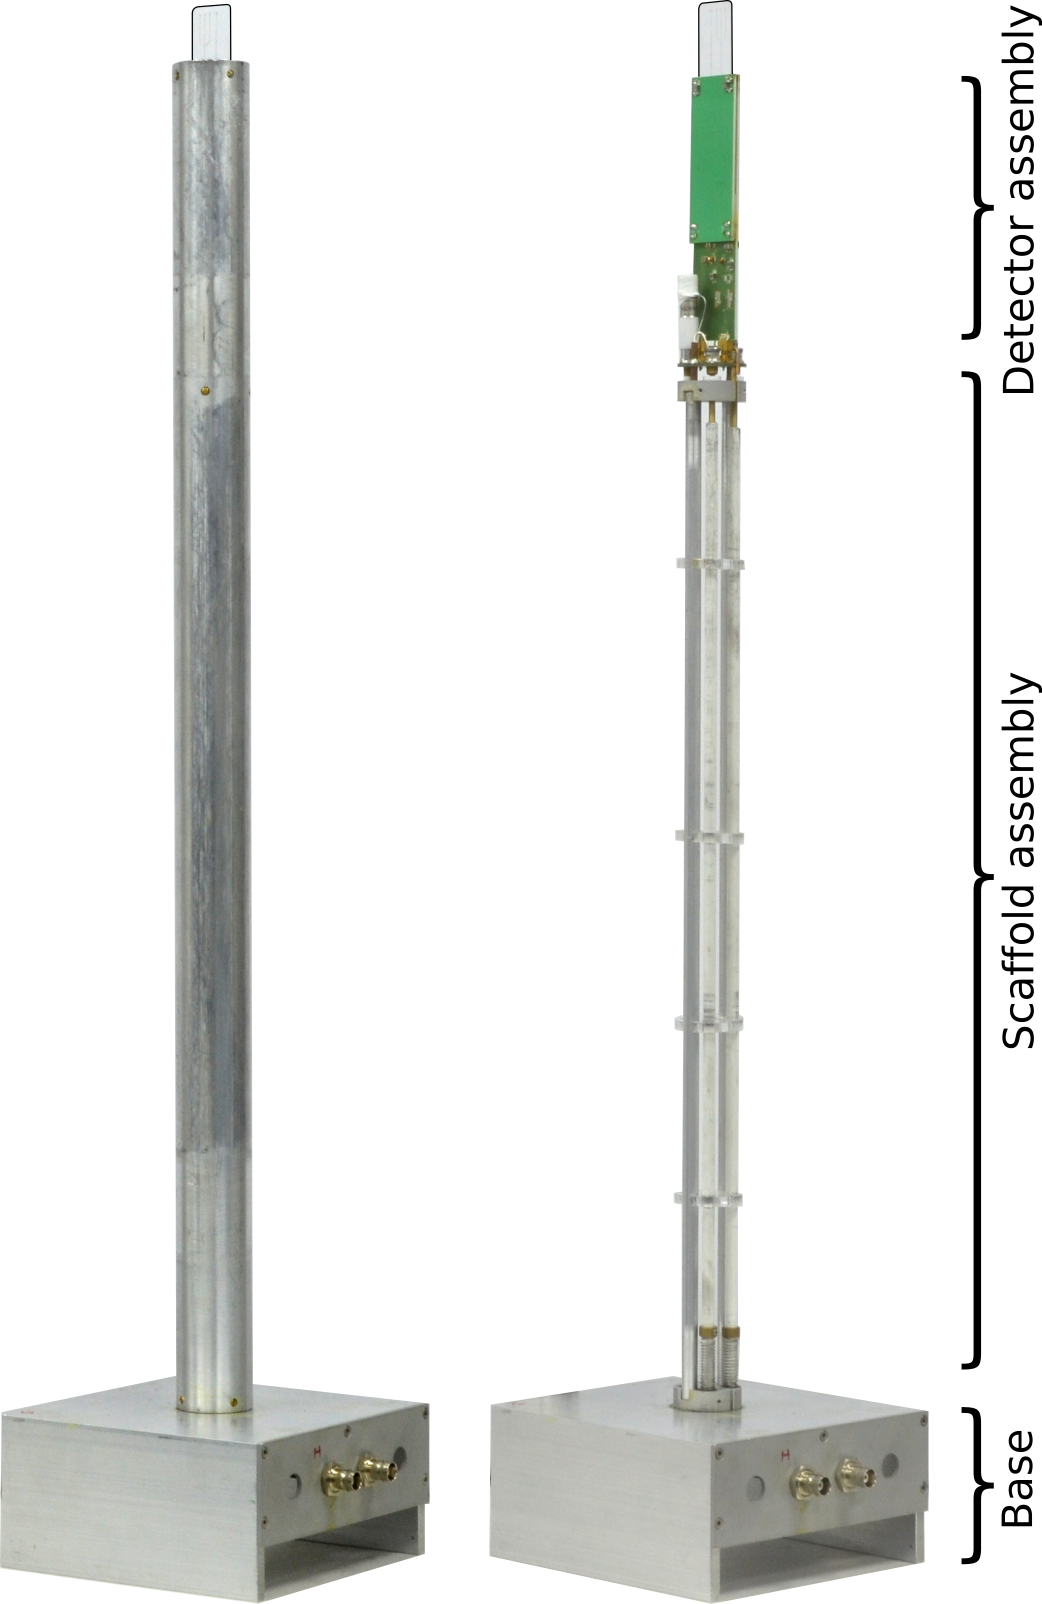
\includegraphics[width=.5\linewidth,keepaspectratio=true]{./figures/ms5n17-tlp-im-181218-probe.png} 
\caption{Micrograph of the probe with and without the sleeve.}
\label{fig:probe} 
\end{figure}
The probe assembly design is based on readily and easily available materials and parts 
with minimal need for fabrication of customised parts to avoid any bottlenecks in the 
building process. The probe can be built from scratch with no requirement of any part 
or electronics from commercial NMR probes. 
All parts and electronic components are readily available from commercial sources, 
with the exception of a small number of precision-machined parts which are used 
to hold the assembly together. These can be ordered from commercial prototyping 
manufacturers or machined in-house if mechanical workshop facilities are available.

\begin{figure}
\centering
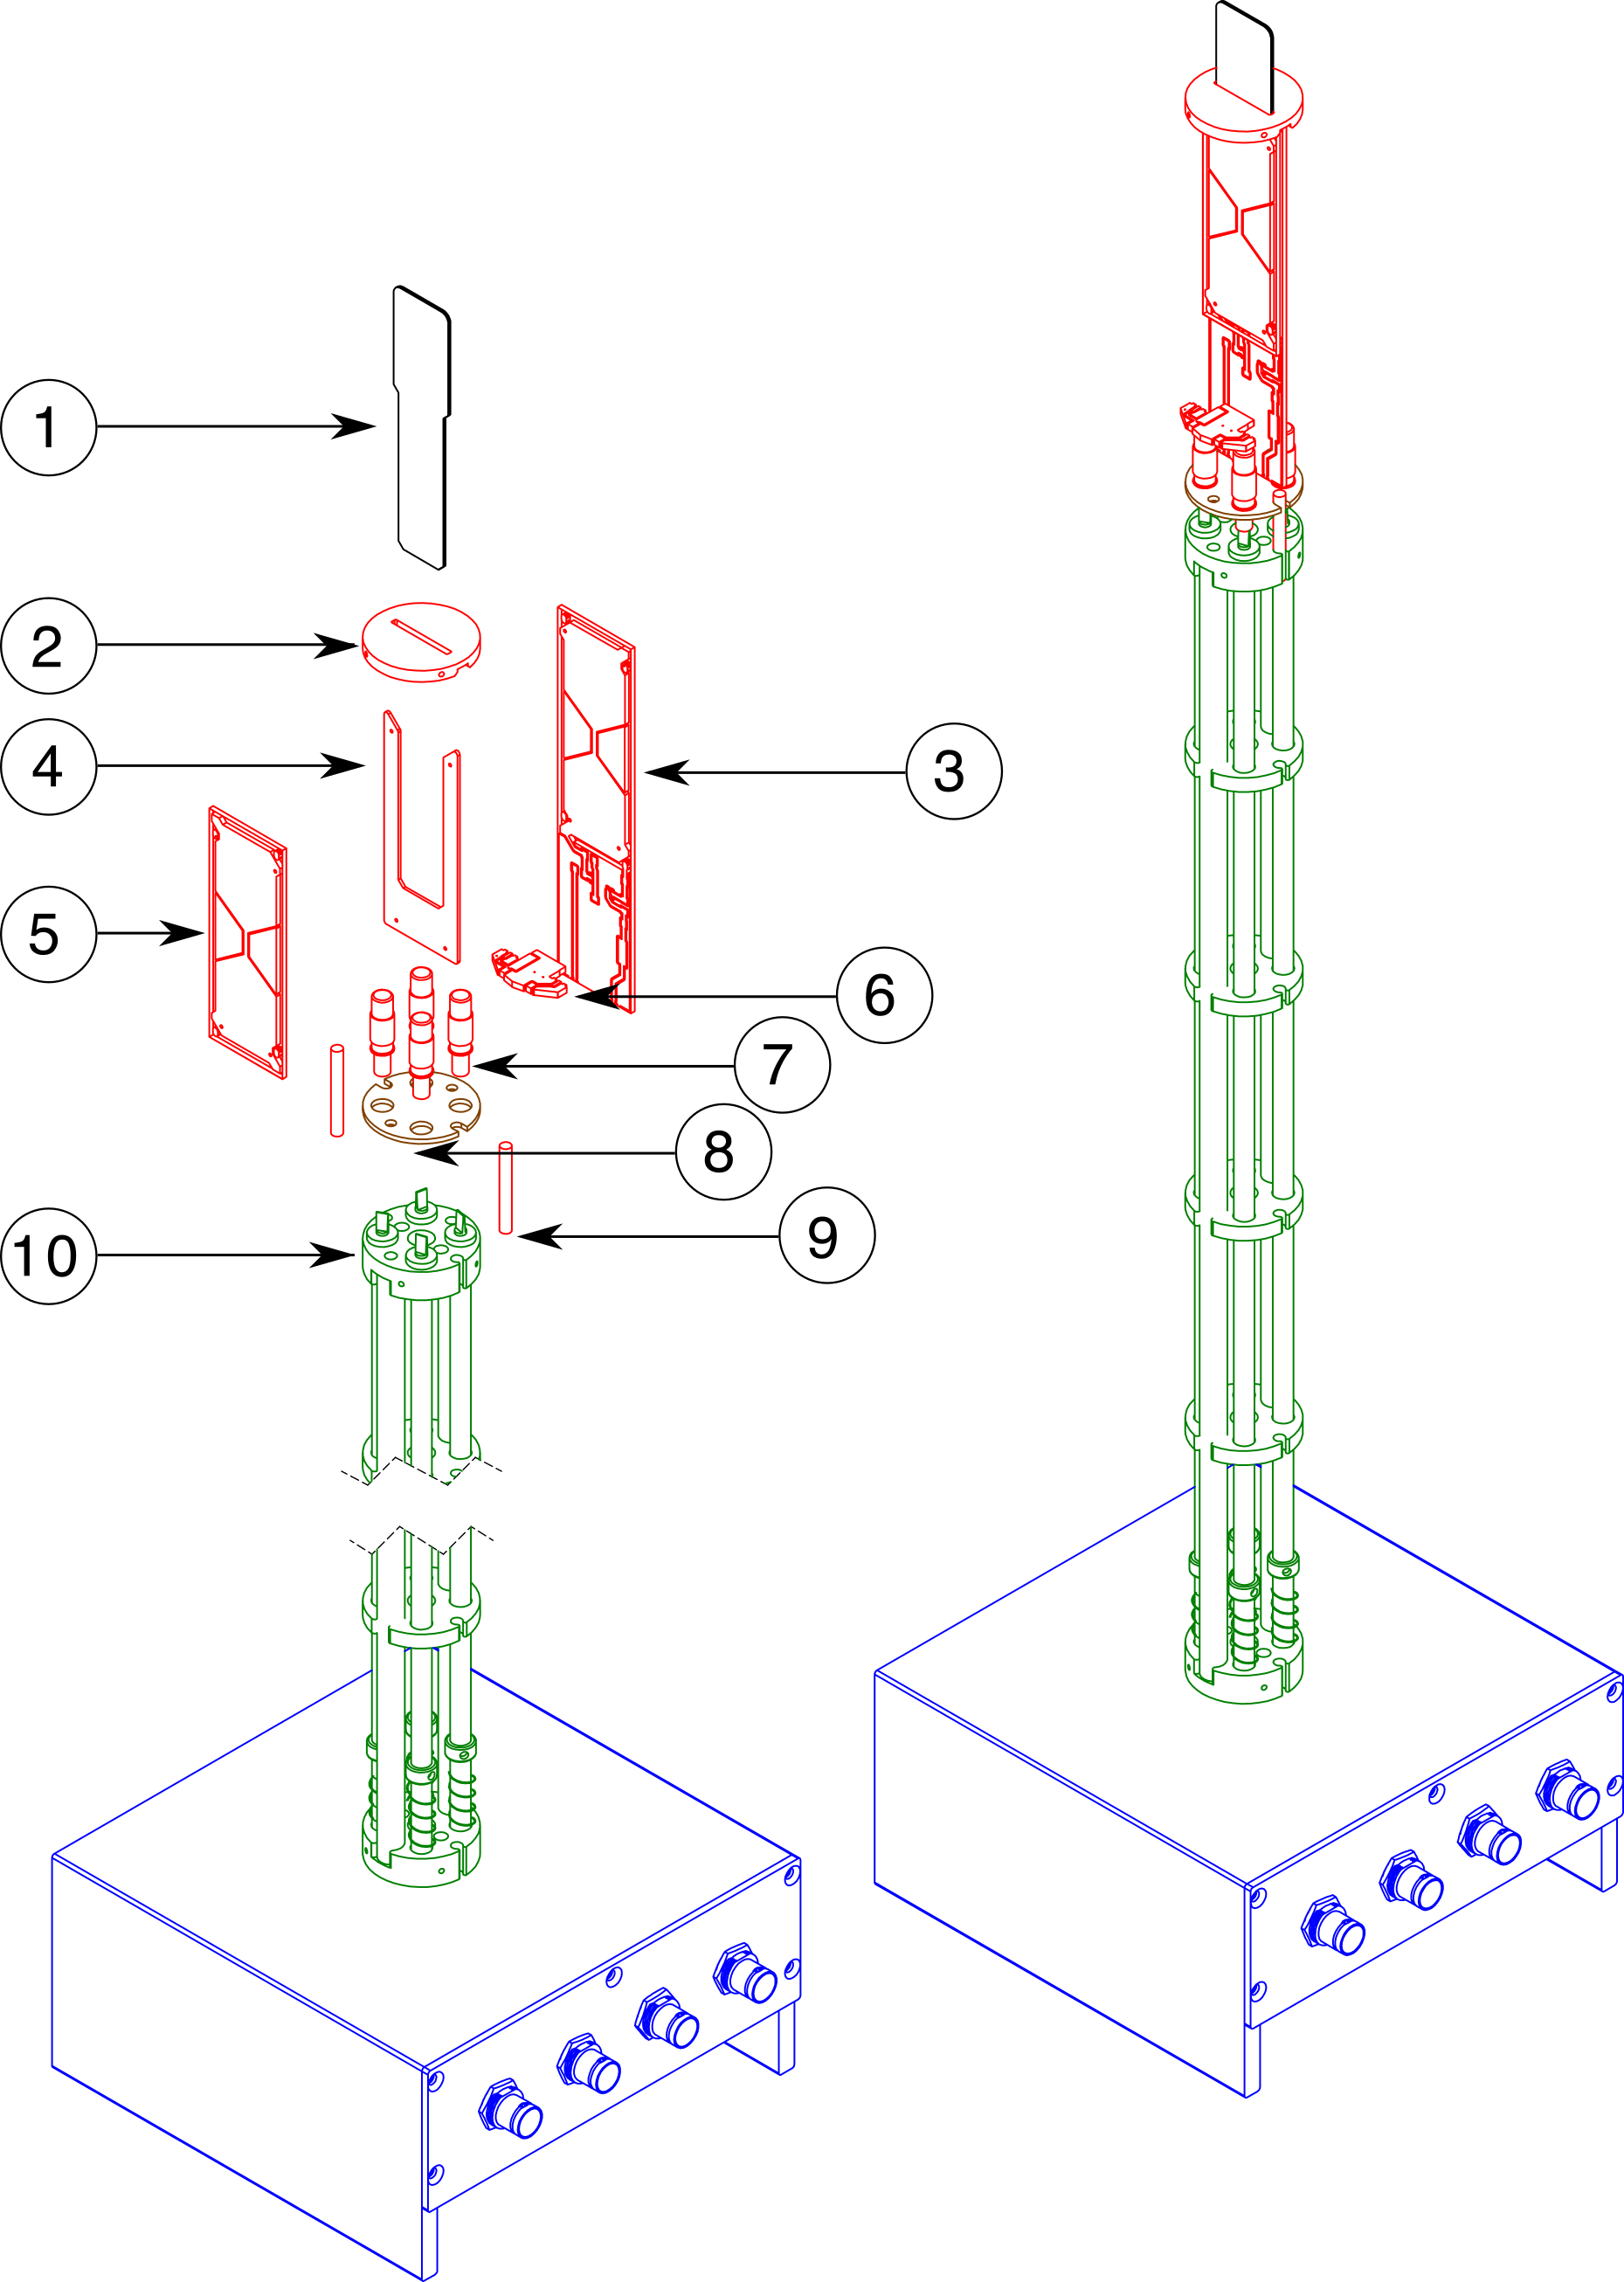
\includegraphics[width=.5\linewidth,keepaspectratio=true]{./figures/ms5n17-tlp-im-181007-Probe-explode.png} 
\caption{Exploded view of he probe design (left) and assembled probe (right). 
Probe base (blue) and scaffold assembly (green) with base PCB (brown, 8) provides a 
generic mounting point for the NMR detector assembly(red). 
A microfluidic device (1) can be inserted from the top of the probe. 
The device is held in place by a spacer (4) between the detector planes (3 and 5) 
ensuring alignment of the sample chamber with the sensitive area on the PCB planes. 
The X channel frequency is controlled by a 
modular PCB insert (6). The modular NMR detector is made up of parts 3 to 6 and is 
connected to the base plate PCB (8) through standard coaxial (SMP) connectors. 
The scaffold assembly is made up of aluminium tubes (11), scaffold support disks (10) 
and, auxiliary support disks (12).}
\label{fig:probe-explode} 
\end{figure}

The probe is composed of three main assemblies: A) probe base; B) scaffold assembly; 
C) detector assembly (figure~\ref{fig:probe}). 
The  base (blue in figure~\ref{fig:probe-explode}) and the scaffold assembly 
(green in figure~\ref{fig:probe-explode}) together make the skeleton of the probe. 
Both the base and scaffold assembly are made from standard aluminium profiles. 
The base contains the BNC connectors for RF (Radio Frequency) input. 
These BNC connectors are connected to semi-rigid coaxial cables for 
RF transport in the probe.

The scaffold assembly is made up of two hollow aluminium tubes (11) held together with 
precision machined parts at either end(scaffold support disks (10)). 
The semi-rigid cables are  threaded through these hollow aluminium tubes 
to reach the detector assembly. 
Auxiliary support disks (12) provide additional rigidity for the scaffold assembly. 
In our case, these were laser cut from 5~mm thick PMMA sheets, 
but they may also be made by conventional machining.
A tuning and matching PCB (TMPCB, 8) is held in place on the top of the probe skeleton by
the detector support rods (9), with the semi-rigid coaxial cables providing
additional support.
The TMPCB is permantly fixed to the probe base, and serves as attachment point
for the exchangeable detector assembly. It also provides 
capacitors (7) for secondary tuning and matching.
The detector assembly is connected to through a pair of
low-loss SMP connectors (14 in figure~\ref{fig:ProbePhoto}).
While each detector assembly is roughly
tuned and matched with fixed circuit elements soldered onto it,
the adjustable capacitors on the TMPCB are used for 
fine tuning and matching 
at the magnet through tuning rods (13) which reach all the way to the probe base. 

The base, the scaffold assembly and the tuning and matching PCB all have a free circular 
axial bore providing access from the bottom of the probe, which can be used for 
temperature and environmental control and/or fluidic connections to the sample as
needed.
The detector assembly is made up of two PCBs (3 and 5), a spacer between them (4) and an 
RF-insert (6). The detector used here is based on a planar transmission line geometry 
as described elsewhere~\cite{gream_2016,stripline_jan}; other structures such as spiral
coils and Helmholtz pairs are also possible, and can easily be realised on a PCB.
The transmission line detector consists of a pair of copper 
planes each with a constriction at the centre.  This geometry gives rise to an 
electromagnetic eigenmode with a strong anti-node of the magetic field between
the two planes at the site of the constriction. This concentrates the rf field 
and the detection snsitivity
onto the sample area. 
The shape and size of the copper structures have been chosen such as to produce
an eigenfrequency of this mode around 630~MHz. The PCBs have been designed with
solder points at the back side for chip capacitors; these can be used to tune the
resonance to the desired proton Larmor frequency (500 or 600~MHz in the present case).
Both the PCBs (3 and 5) also carry circuitry for the channel separation and primary 
tuning and matching of the detector. A copper or brass auxiliary disk (2) holds the PCBs 
together. 
The probe sheath (not shown here) is connected to the auxiliary disk (2) 
and the scaffold assembly through screws. 
An exchangeable microfluidic device (1) can be inserted from the top of the detector. 
Microfluidic devices can be used as passive sample holders, filled before putting them
into the probe,
or the device can be actively perfused and operated in-situ, with fluidic connections 
attached inside the magnet. The microfluidic device is held in place by the spacer 
between the two PCB planes coinciding the sample chamber with the constriction on the 
detector.  The 45-degree edges of the device outline help with precise and reliable
alignment. 

The RF-insert (6) can be exchanged to tune and match the probe to different frequencies 
at the X channel. As the detector is connected to the probe base through detachable 
connectors, various detectors can be used on the same probe skeleton. 
Using standard PCB processes to manufacture the detector provides great flexibility
to optimise detector performance for different applications, including different
microfluidic sample sizes, and different combinations of target nuclei.
\par
\begin{figure}
\centering
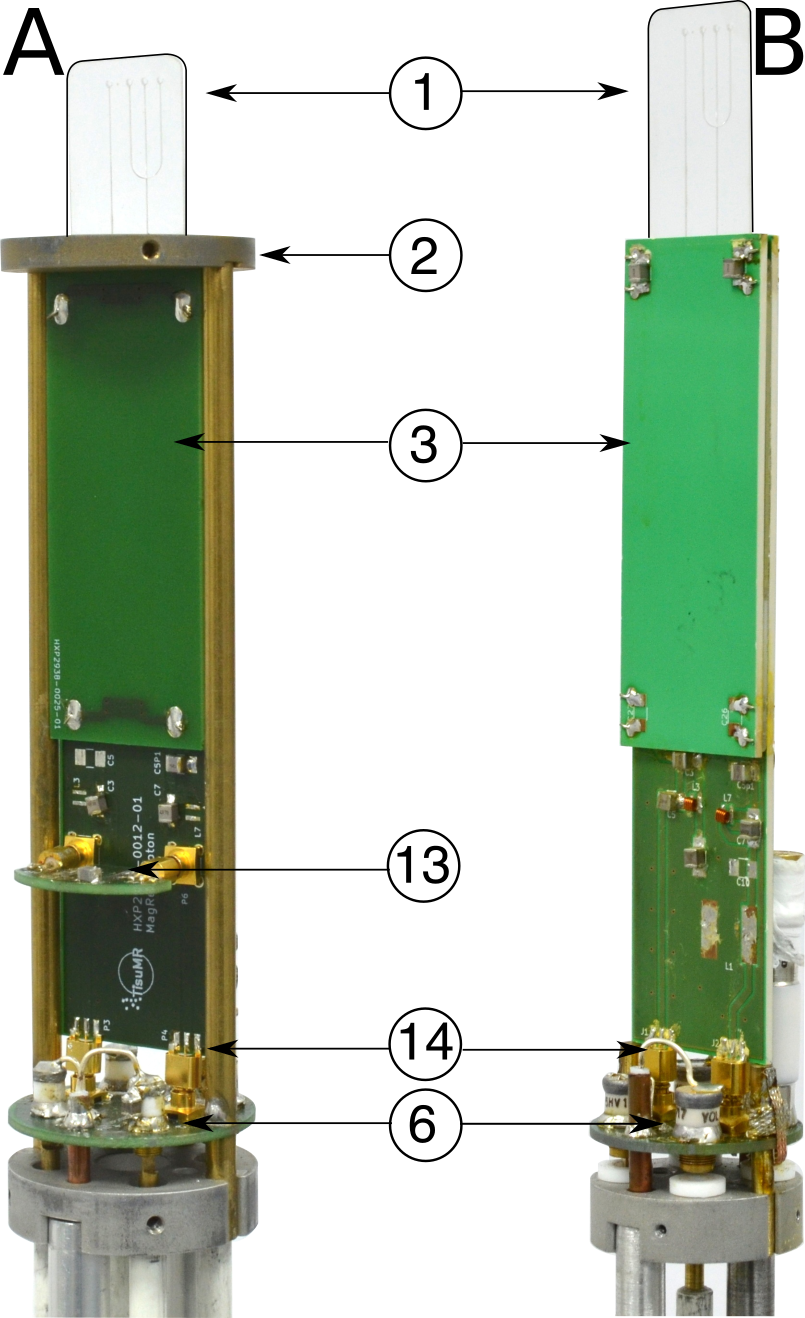
\includegraphics[width=.5\linewidth,keepaspectratio=true]{./figures/ms5n17-tlp-im-181007-both-detectors.png}
\caption{Dual channel probes with (A) and without (B) modular RF insert (6) for X channel. A has an O.D. of 44.45 mm, in B, circuit elements of X channel are integrated on the PCB itself making it compact (38 mm O.D.). Detachable SMP connectors (14) are used to connect the RF insert (6) and also the assembled NMR detector. The cost and effort to make a new detector are minimal so, various detectors could be made for various X channel frequencies.}
\label{fig:ProbePhoto}
\end{figure}
Figure~\ref{fig:ProbePhoto} shows two different versions of the probe with and without the RF insert (6) for the X channel. In (A) the X channel can be tuned to different nuclei by exchanging 6. However, in (B) the circuitry of the RF insert (6) is manufactured on the PCB plane (5). Inclusion of the circuitry of 6 on 5 makes the design more compact. Probe (A) is compatible with Varian 600 ultra shield 14.1 T magnet having an outer diameter (O.D.) of 44.45 mm including the sheath. Probe (B), with an outer diameter (O.D.) of 38 mm including the sheath, is designed to fit inside a Bruker narrow bore shim stack. Probe (B) also fits inside a Bruker micro-imaging gradient unit. Naturally, B can also be used with wide bore magnets with spacers or gradient stack to keep the probe centred .\par
The microfluidic devices are made from thermally bonded PMMA sheets. The sample chamber and fluidic network are made in the middle layer. The middle layer is sealed in between the bottom and the top layers with inlet and outlet in the top layer. A flow can be introduced from the inlet and outlet of the device for flow studies or sample exchange. The fluidic network on the device can be made freely with the only constrained on the overall size of the device. Other layers can be employed to allow parallel flow as long as the total thickness remains below 1mm.\par
\begin{figure}
\centering
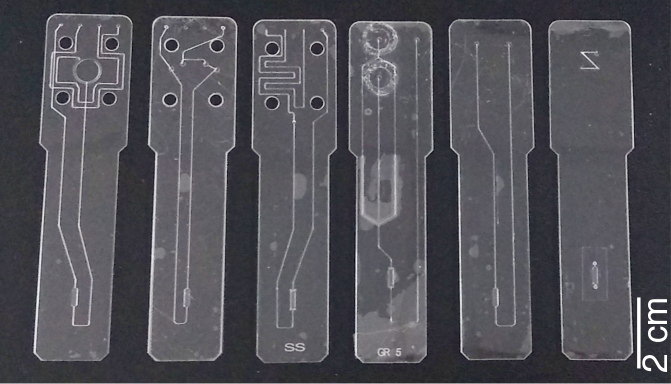
\includegraphics[width=.7\linewidth,keepaspectratio=true]{./figures/ms5n17-tlp-im-181007-devices.png} 
\caption{Microfluidic devices for different applications compatible with the current setup. From left: Devices for perfusion of tissue slice on a chip, peristaltic pumping to induce flow, hydrogenation on a chip, droplet generator, simple design to fill the sample chamber and, to grow cells on the device.}
\label{fig:device} 
\end{figure}
The circuit for a double resonance probe is based on design shown in figure~\ref{fig:circuit}. The size of the constriction was larger compared to~\cite{gream_2016} to allow use of larger sample volumes for some cases. Primary tuning of the detector is performed through the circuit elements (mainly C$_6$). The detector is connected to the secondary tuning and matching capacitors with the transmission lines on the PCB planes. As all the circuit elements are assembled on the PCB planes, the transmission lines on the PCB have lengths similar to the detector. Hence transmission lines may become a part of the resonance circuit and can severely affect the probe performance. To avoid this problem a series capacitor (C$_5$) was included with the transmission line just before the detector to adjust the impedance of transmission line to 50~$\Omega$. In this situation the detector is matched by the transmission line and secondary tuning and matching capacitors can be used for fine tuning and matching.\par
\begin{figure}
\centering
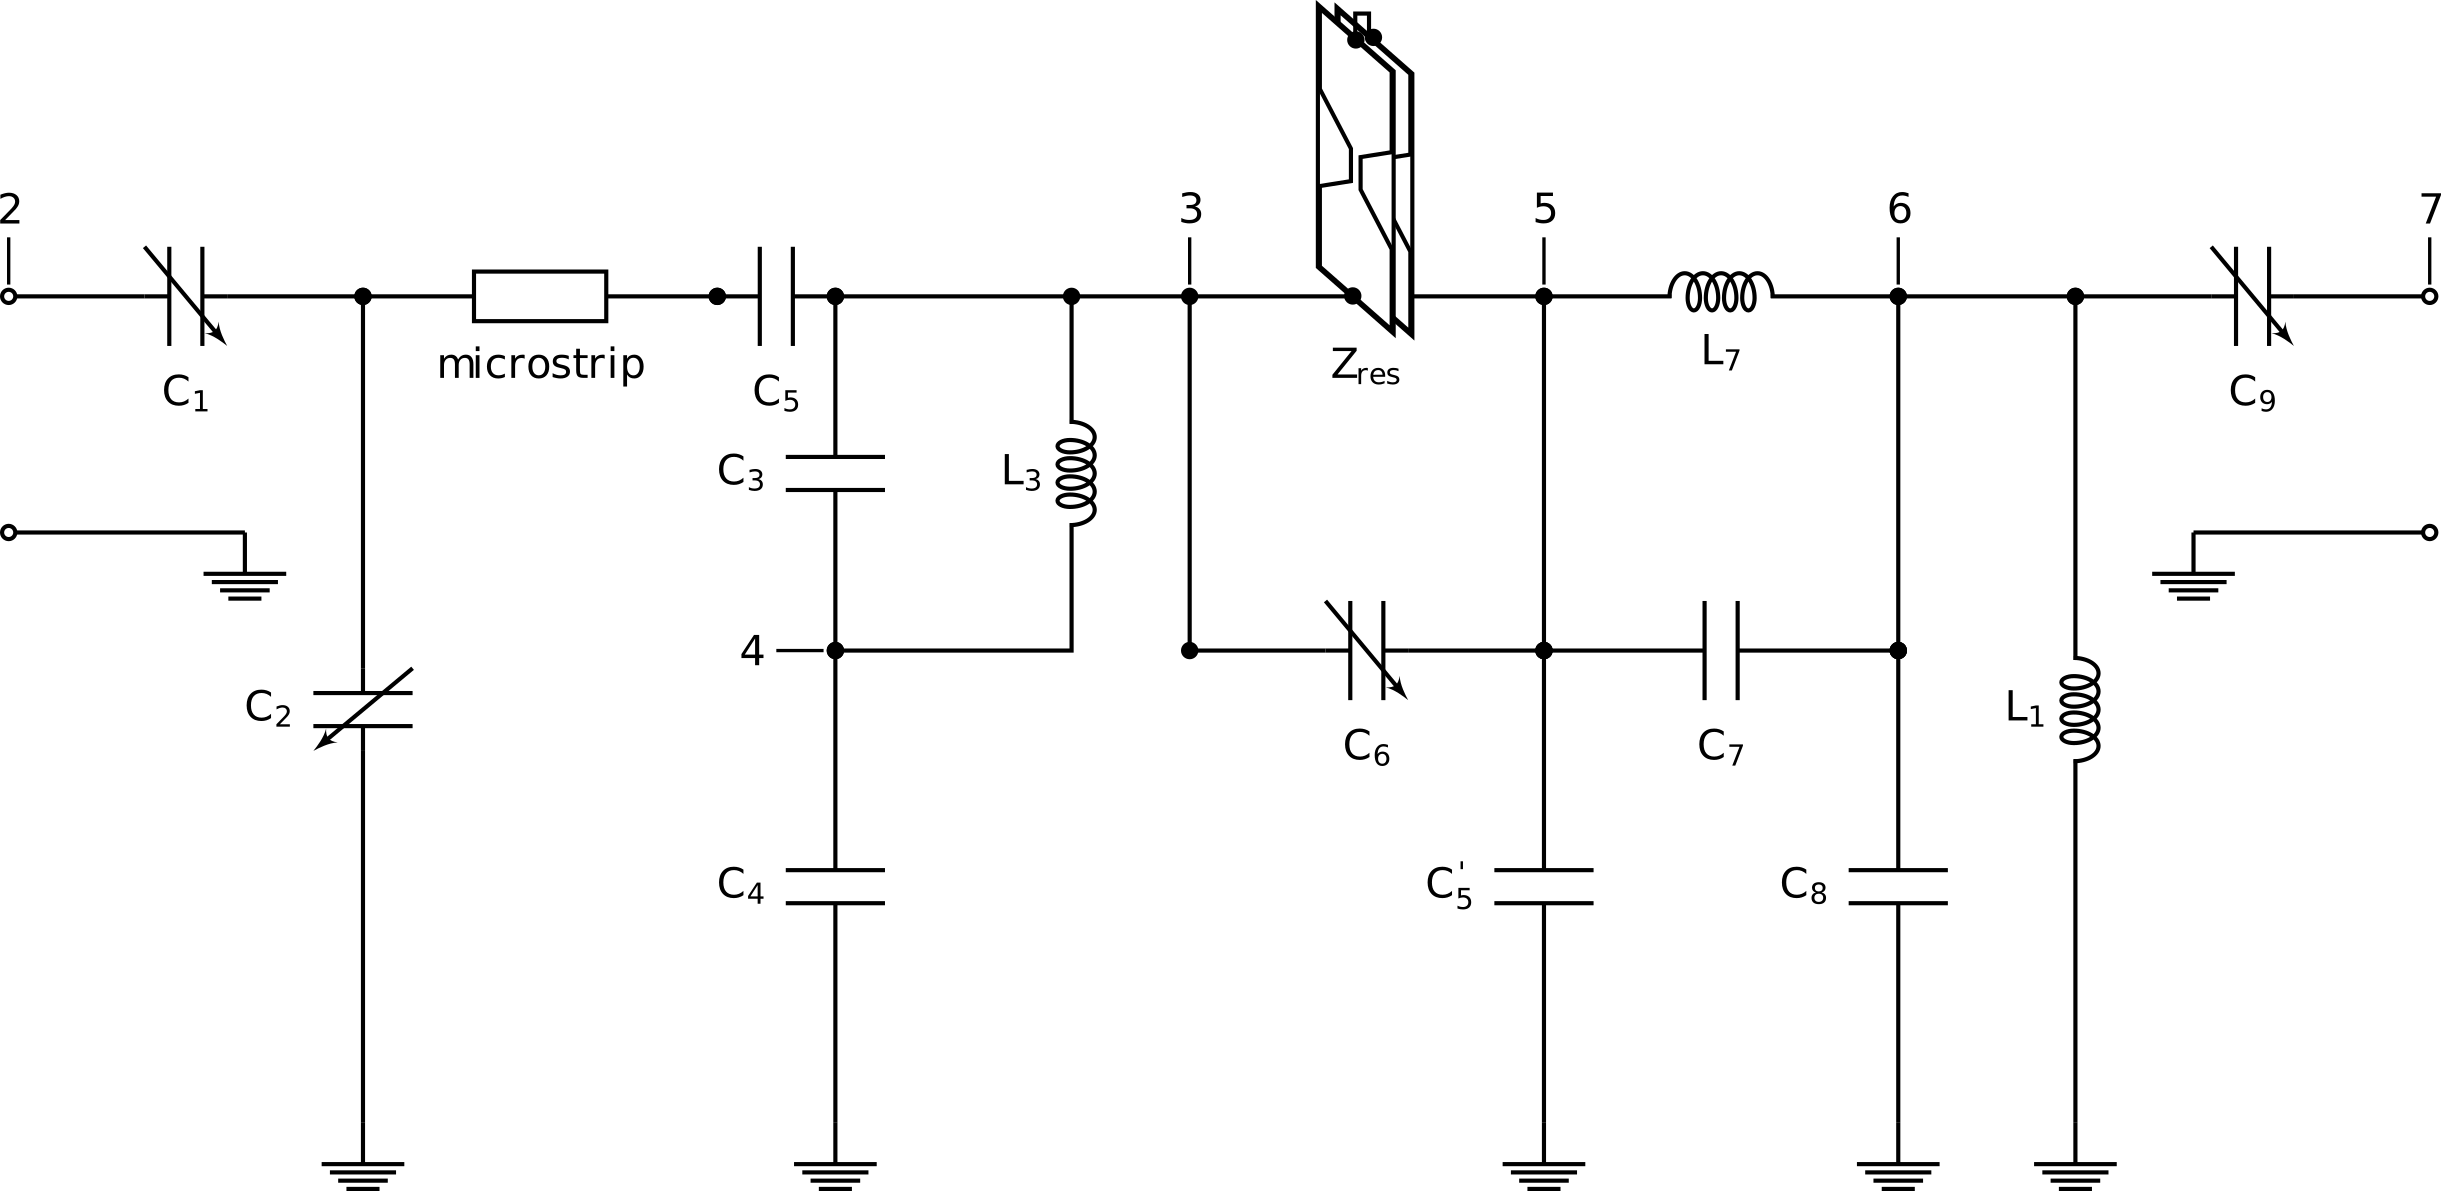
\includegraphics[width=.7\linewidth,keepaspectratio=true]{./figures/ms5n17-tlp-im-180110-circuit-diagram.png}
\caption{Circuit diagram of the double resonance probe. Proton frequency is feed in from the left (port 2) and X frequency is feed in from right (port 7).}
\label{fig:circuit}
\end{figure}
%%%%%%%%%%%%%%%%%%%%%%%%%%%%%%%%%%%%%%%%%%%%%%%%%%%%%%%%%%%%%%%%%
\section{Materials and Methods}
%\begin{itemize}
%	\item Design process (SolidWorks, etc)
%	\item Manufacture of parts (ProtoLabs, some in-house machining)
%	\item Optimisation of resonator geometry (ref Graeme's paper)
%	\item Design and optimisation of tuning/matching circuitry (Mathematica routines)
%	\item Design of PCB using KiCAD
%	\item PCB material and manufacture
%	\item Assembly, soldering
%	\item NMR spectrometers and parameters
%	\item samples
%\end{itemize}
%The probe base platform is made up of 6 mm thick aluminium sheet [$l\times w \times h = 150 mm\times 150mm\times 75mm$]. Probe sleeve has diameter of 38 mm compatible with Bruker 500 MHz. The probe was used with a spacer on varian 600 MHz.
All the parts and the probe assembly were designed and simulated on Solidworks (Solidworks, Dassault Syst\`{e}mes). The prefabricated aluminium profiles (base platform, scaffold aluminium tubes, probe sleeve) were made from 6061-T3 alloy and were obtained from Aluminum Warehouse, UK to build the probe skeleton. A few customised precision-machined parts (scaffold support disks, top disk) were obtained from ProtoLabs (Telford, UK) after providing CAD files. A small number parts were machined in-house (detector support rods, auxiliary support disks). All the electronic components and the semi rigid transmission lines were purchased from Digikey. Cell cast PMMA sheets for microfluidic devices were bought from Weatherall Equipment (Wendover, UK). Microfluidic devices were designed on AutoCAD. PMMA sheets were cut to desired size and functionality (holes or channels) through a laser cutter (HPC Laser L3040). The fluidic channels were cut or scored in a 0.5 mm thickness PMMA sheet. The device is made by thermally bonding PMMA sheets using the protocol described in~\cite{yilmaz_bonding}.\par
Dimensions of the detector were calculated from the simulation described in~\cite{gream_2016}. The probe circuit for the double resonance probe was simulated on Mathematica using a symbolic analysis network code to asses the performance of both the channels~\cite{gream-thesis}.\par
The probe circuit was compiled in KiCAD to design the PCB layout. The PCB layout was provided to beta-layout (Aarbergen Germany) and P.W. Circuits LTD (Wigston , UK) to manufacture the PCBs. Easily and inexpensively available FR4 was used for PCB manufacturing for (figure~\ref{fig:ProbePhoto} A). RO3035 from Rogers corporation was used for PCBs used in (figure~\ref{fig:ProbePhoto} B).\par
The probe skeleton was assembled by holding the prefabricated aluminium profiles with precision-machined parts and screws. Semi-rigid transmission lines were then threaded through the skeleton. The base PCB plate was soldered on top of the semi-rigid transmission lines. The detector planes (3 and 5) were soldered together separately with the required electronic components characterise by network analysis. Minor changes were made to the values of the probe electronic components to optimise the probe performance in practise.\par
NMR experiments were performed on Varian VNMRS console on a Varian 600 ultra shield 14.1 T magnet. Spectra in figure~\ref{fig:lineshape} and \ref{fig:media-spec} were obtained with water presaturation followed by a 90$^{\circ}$ pulse. Spectrum in figure~\ref{fig:1H-nutation} was acquired with increasing the pulse length. Spectrum in figure~\ref{fig:15N-nutation} was acquired using pulse sequence described in~\cite{bax_indirect}. Sodium acetate and $^{15}$N labeled urea were purchased from Merek and Dulbecco Modified Eagle's Medium (DMEM) supplemented was purchased from Life Technologies, USA.\par
Imaging experiments were performed on Bruker AVANCE III spectrometer on a Bruker Active Shield II wide bore 11.7 T magnet. To obtain the tissue slices first a core of 8 mm diameter was extracted using a biopsy punch from the liver. PCLS of thickness 250-300 $\mu$m were prepared using a Krumdieck Tissue slicer. Circular slices of 3 mm diameter were then cut from this slice using a smaller punch.The slices were put in the incubator for 2 hours before imaging to allow equilibrium.
%%%%%%%%%%%%%%%%%%%%%%%%%%%%%%%%%%%%%%%%%%%%%%%%%%%%%%%%%%%%%%%%%%
\section{Results and Discussion}
%\begin{itemize}
%	\item Tuning/matching/channel separation
%	\item tuning range (different field strengths)
%	\item Sensitivity calibration
%	\item Resolution
%	\item RF efficiency, B1 homogeneity
%	\item Example spectra to illustrate versatility:
%		\begin{itemize}
%		\item Growth media (1H), cell culture
%		\item Comparison of spectra obtained at 300, 500, 600 MHz
%		\item HSQC (13C, 15N)
%		\item Liver slice image
%		\end{itemize}
%\end{itemize}
A double channel probe allows heteronuclear NMR experiments which are essential for many applications like protein structure determination. The current probe can be simultaneously operated at 2 frequencies. The probe can be tuned to protons and one X channel ($^{13}$C or $^{15}$N) frequencies at a time. As already explained, the X channel tuning frequency can be changed by simply exchanging an rf-insert or the complete detector. Figure~\ref{fig:tandm} shows the measured tuning and matching curves at different proton (600 MHz, 500 MHz) and X channel frequencies (60 MHz and 125 MHz) corresponding to the larmor frequencies of $^{15}$N and $^{13}$C at magnetic fields of 14 T and 11.7 T respectively. The measurements were performed in the pairs of 600 MHz and 60 MHz and, 500 MHz and 125 MHz. The loaded Q factors are 42, 49, 32, 36 at 600 MHz, 500 MHz, 125 MHz and, 60 MHz respectively. Channel separation is better than 15 decibels at all operating frequencies and thus sufficient to perform decoupling during experiments.\par
\begin{figure}
\centering
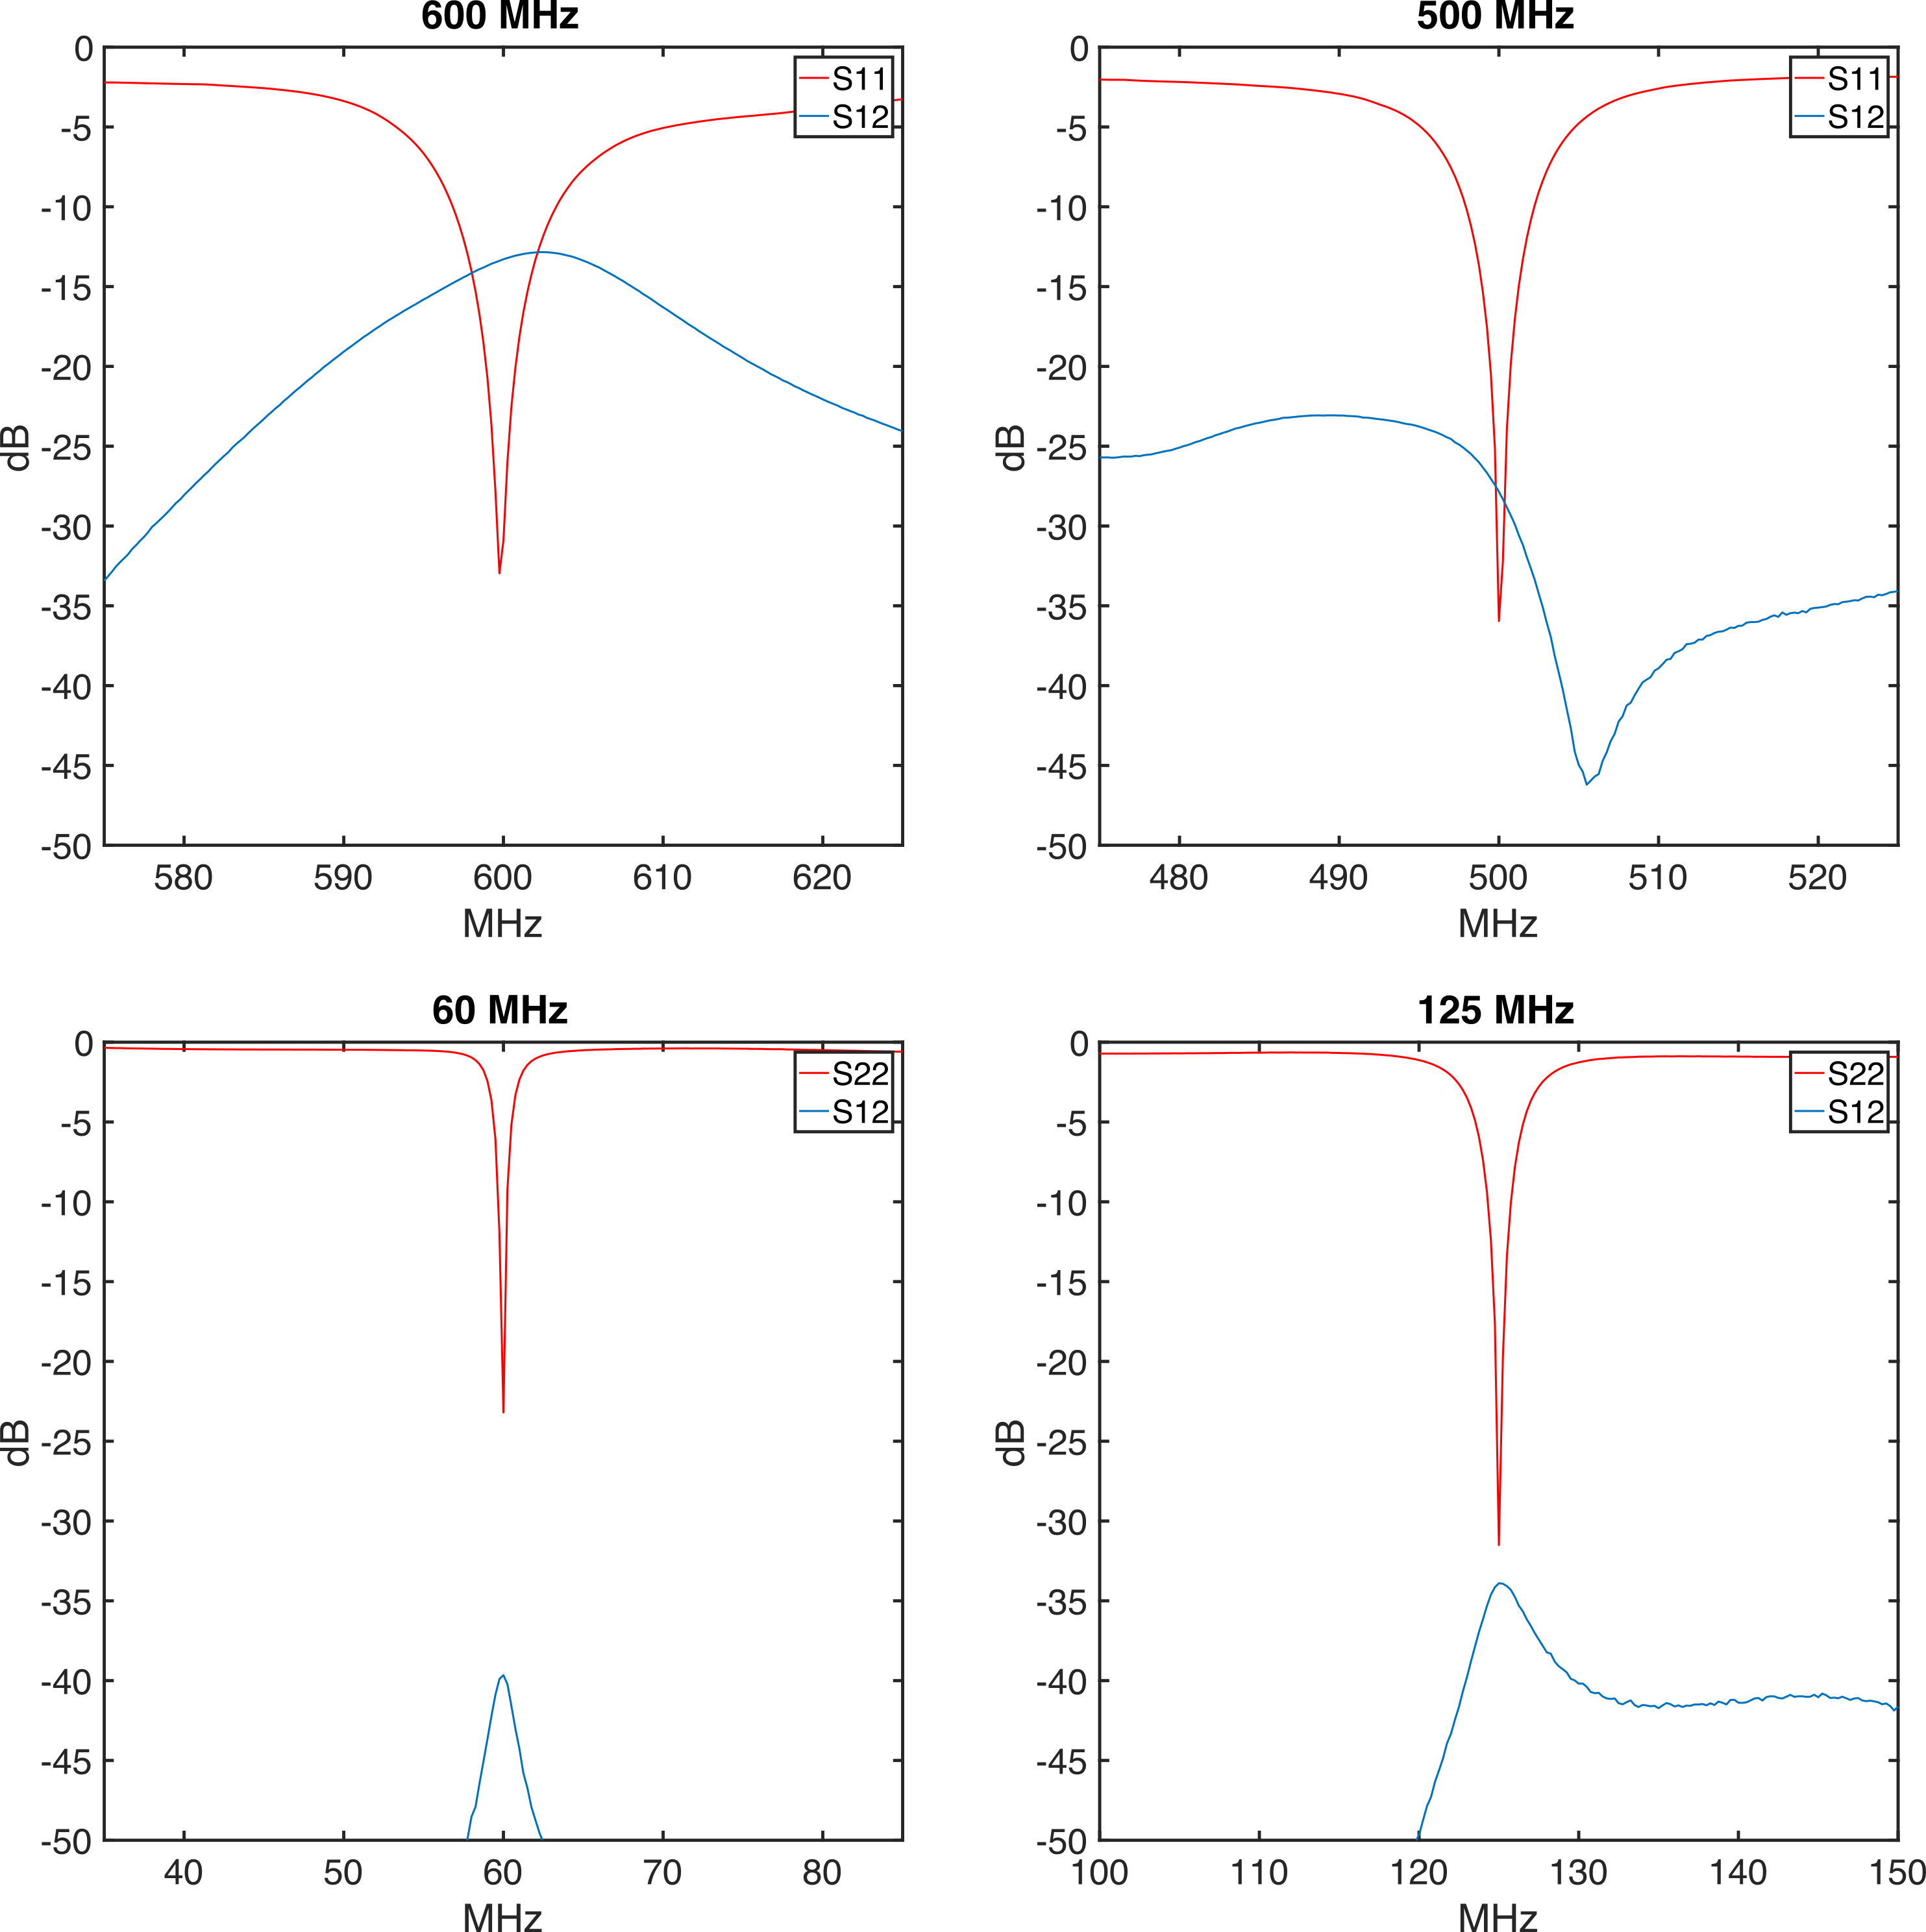
\includegraphics[width=.7\linewidth,keepaspectratio=true]{./figures/ms5n17-tlp-im-180710-tandm-sameaxis.png} 
\caption{Experimental tuning and matching curves measured at 600 MHz, 500 MHz, 60 MHz ($^{15}$N frequency at 14 T) and, 125 MHz ($^{13}$C frequency at  and 11.7 T). Probe can be tuned to 2 frequencies at a time, above results were measured in pairs of 600 MHz with 60 MHz and 500 MHz with125 MHz. Decoupling can be performed at all the frequencies as the channel separation is better than 15 decibels at all frequencies.}
\label{fig:tandm} 
\end{figure}
Initially FR4 PCB material was used to make detector assembly because of its low cost and easy availability. B$_0$ field maps of the sample chamber generated from gradient echo images using these detectors showed inhomogeneities in the B$_0$ field. To avoid inhomogeneities and therefore to achieve better resolution, detectors were made from RO3035 material from Rogers corporation. Though RO3035 provides better resolution it is more expensive and takes longer to obtain compared to FR4. A new detector design can first be tested using FR4 material and the optimised design can be made from RO3035.\par
$^1$H nutation diagram of water peak for a sample of 100 mM $^{15}$N-urea dissolved in water measured at 600 MHz is shown figure~\ref{fig:1H-nutation}. RF field is highly homogeneous with 810$^{\circ}$/90$^{\circ}$ ratio of more than 90\% at 600~MHz. The probe can generate 100 kHz RF-field for an input power of 100 W both at 600 MHz and 500 MHz corresponding to RF field efficiency (B$_{1}/\sqrt{power}$) of 10 kHz/$\sqrt{W}$ . $^{15}$N nutation detected on protons for the same sample is shown in figure~\ref{fig:15N-nutation}. An RF field of 6 kHz at 60 MHz can be generated at 14 T for $^{15}$N and an RF field of 14 kHz at 125 MHz can be generated at 11.7 T for $^{13}$C with measurements. The power used at the X channel was more than 100 W still no signs of arcing were observed in the NMR spectrum.\par
\begin{figure}
\centering
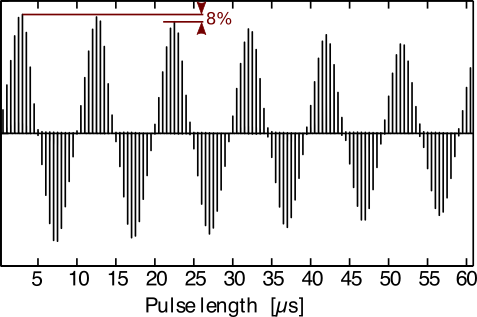
\includegraphics[width=.7\linewidth,keepaspectratio=true]{./figures/ms5n17-tlp-sp-150218-1-Hnutation-171216-103.png} 
\caption{$^1$H nutation acquired for water peak from a sample of 100 mM $^{15}$N-urea dissolved in water measured at 600 MHz. The 810$^{\circ}$/90$^{\circ}$ ratio is more than 90\% at 600~MHz. The 90$^{\circ}$ pulse length is below 2.5 $\mu$ sec corresponding to 100 kHz radio-frequency field for an input power of 100 W. Similar B$_{1}$ efficiency and homogeneity was observed at 500 MHz}
\label{fig:1H-nutation} 
\end{figure}
\begin{figure}
\centering

\includegraphics[width=.7\linewidth,keepaspectratio=true]{./figures/ms5n17-tlp-sp-150218-15-Nnutation-171215-003.png} 
\caption{$^{15}$N nutation detected on proton of $^{15}$N-urea dissolved in water acquired at 14 T corresponding to 60 MHz frequency. A radio-frequency field of 6~kHz can be generated at 60~MHz.}
\label{fig:15N-nutation} 
\end{figure}
Figure~\ref{fig:lineshape} shows a spectrum of 130 mM Na-acetate peak dissolved in H$_2$O acquired after water presaturation at 600 MHz with 32 averages. The figure in the inset shows expanded view of the base of the acetate peak. Carbon satellites can be seen well above noise level. The orange curve corresponds to a Lorentzian lineshape with full width at half maximum of 3.35 Hz. Limit of detection $nLOD_{\omega}=\frac{3n\sqrt{{\Delta}t}}{SNR}$ is  1.18 nmol s$^{1/2}$ at 600 MHz for the acetate sample. The measured LOD is found to be better than the calculated LOD in~\cite{gream_2016} for 600 MHz.\par
\begin{figure}
\centering
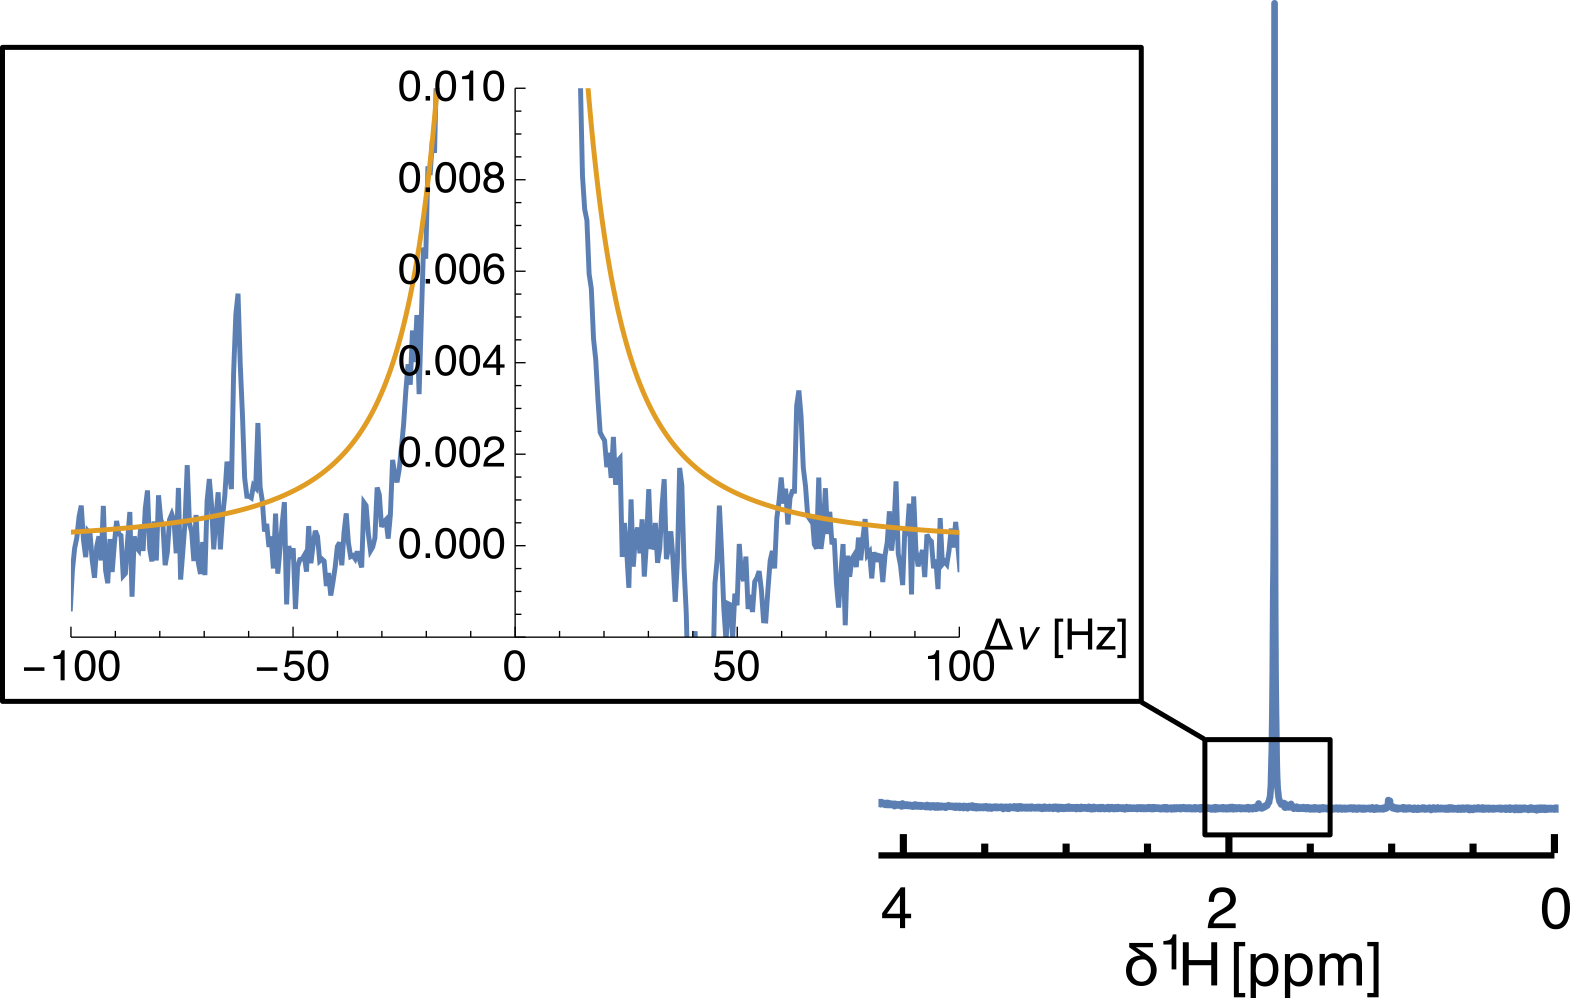
\includegraphics[width=.7\linewidth,keepaspectratio=true]{./figures/lineshape.png} 
\caption{Spectrum of 130 mM sodium acetate dissolved in water acquired in 32 scans with water presaturation. Carbon satellites can be seen in the expanded base of the acetate line. The orange curve shows a lorentzian lineshape with full width at half maximum of 3.35 Hz.}
\label{fig:lineshape} 
\end{figure}
Though the resolution for the current setup is not optimised, it can be used to acquired spectrum with sufficient resolution to differentiate between peaks of different molecules in a mixture. Spectrum of DMEM (Dulbecco's modified Eagle's medium) cell growth media acquired with 256 scans in 20 mins is shown in figure~\ref{fig:media-spec} to demonstrate the feasibility of acquiring spectrum for metabolomic studies. Figure~\ref{fig:HSQC} shows the possibility of useful double resonance experiments in the current setup. On left, $^{13}$C-$^{1}$H-HSQC spectrum, acquired in 12 mins (32 t$_1$ increments and 16 scans) from 2.5 $\mu$l sample of 100 mM $^{13}$C-glucose dissolved in water. On right, $^{15}$N-$^{1}$H-HSQC spectrum, acquired in 400 mins (64 t$_1$ increments and 128 scans) from 2.5 $\mu$l sample of 1 mM $^{15}$N-ubiquitin (17 $\mu$g) dissolved in a buffer solution. $^{15}$N is a very insensitive nuclei hence very difficult to detect. $^{15}$N-$^{1}$H-HSQC spectrum on 1 mM of protein sample clearly shows that the current probe can be used for protein structure studies with minimal amount of isotopically labeled protein.\par
\begin{figure}
\centering
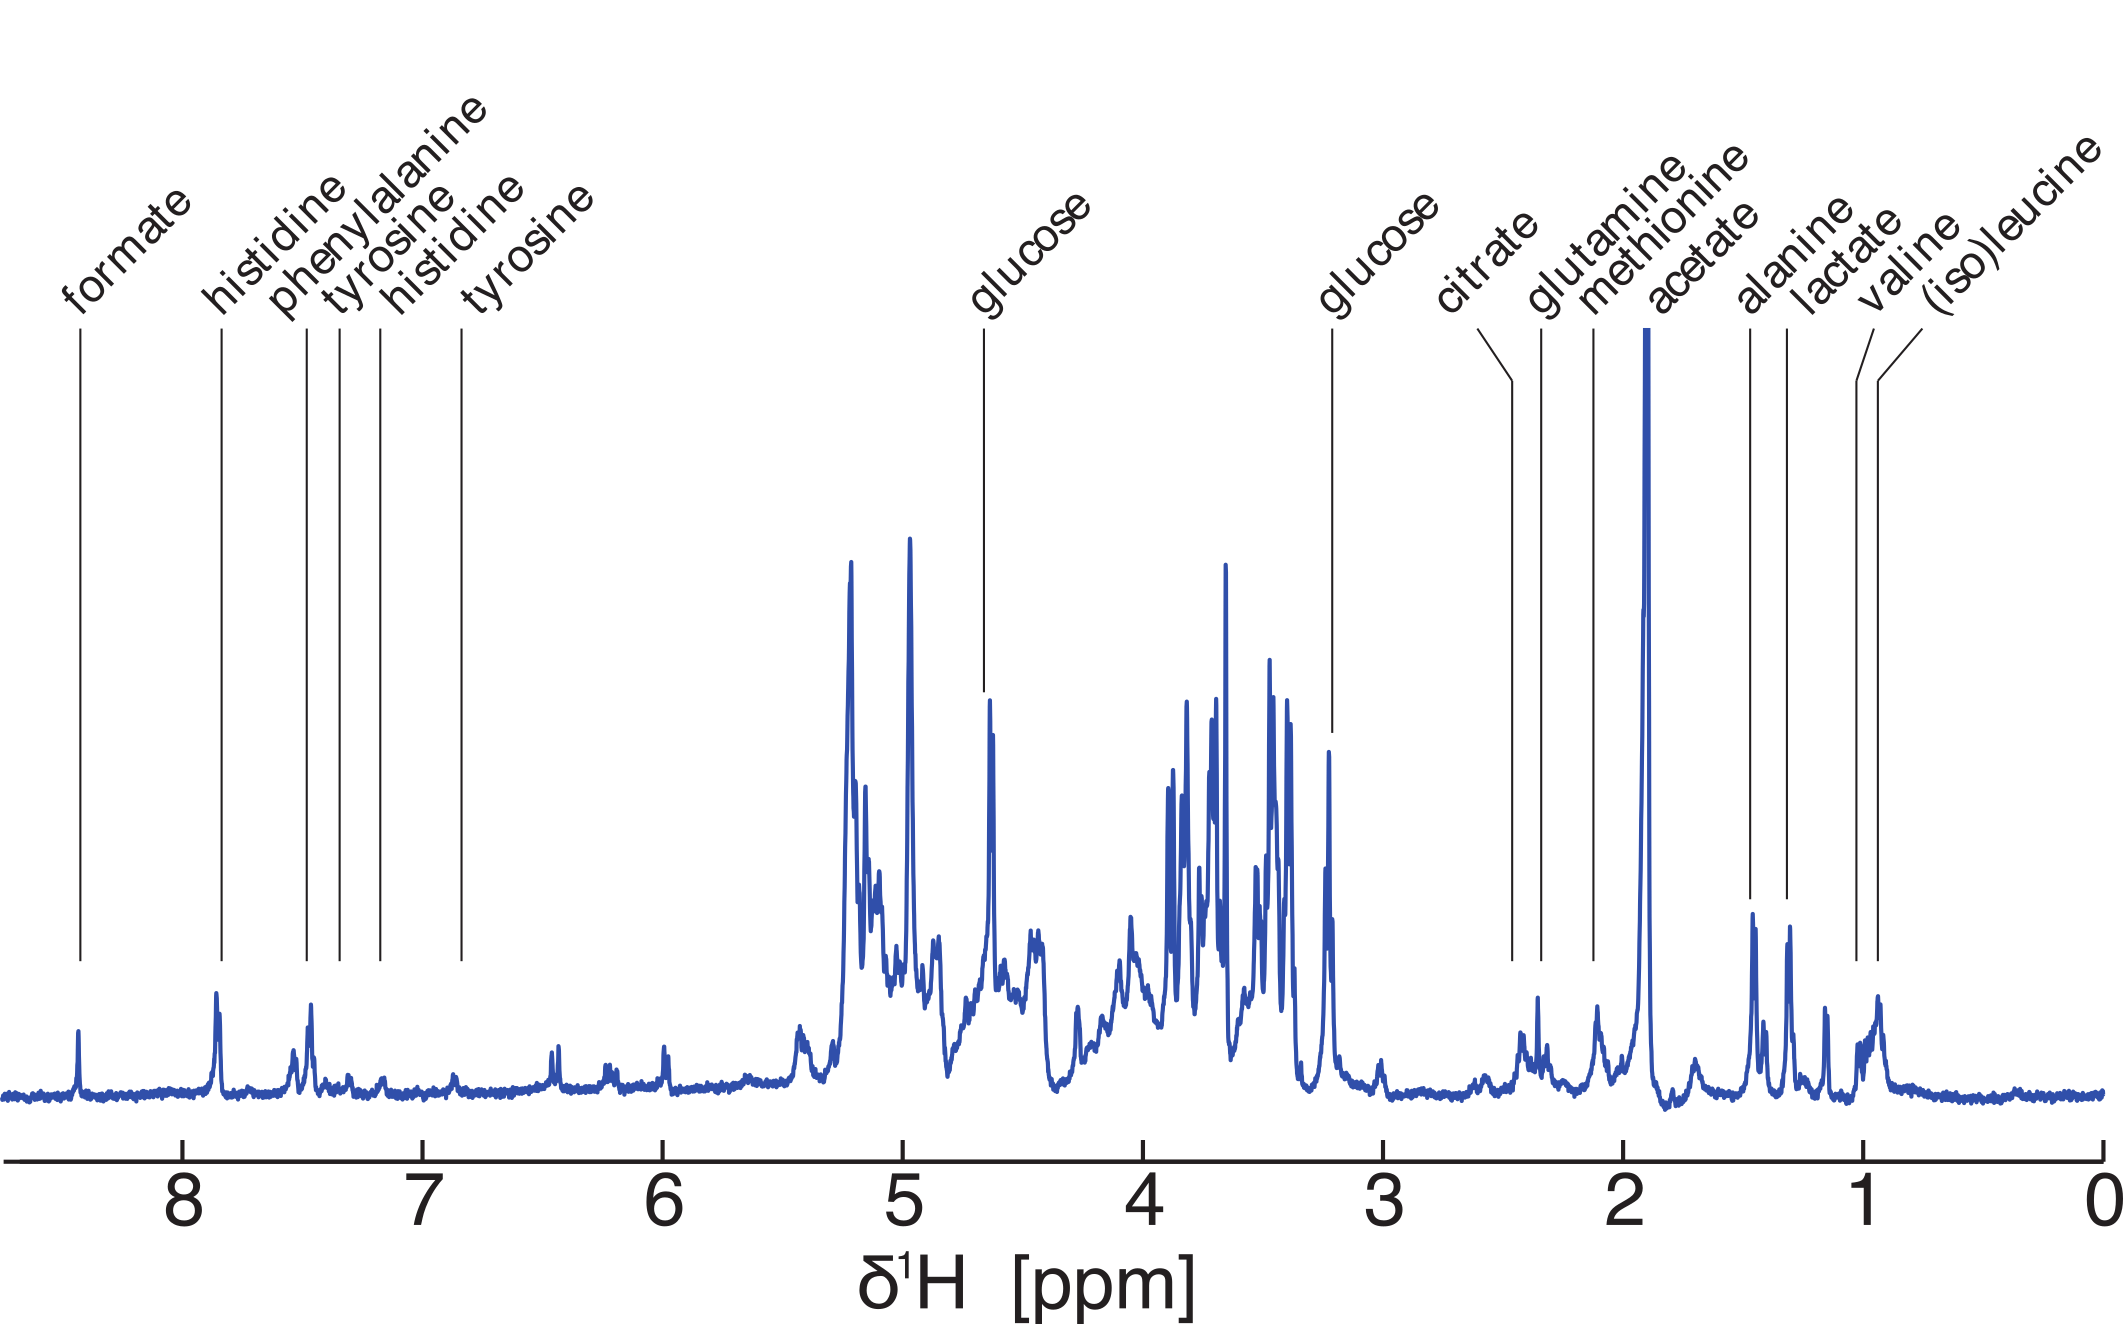
\includegraphics[width=.7\linewidth,keepaspectratio=true]{./figures/media-180125-005-bigger-font.png} 
\caption{Spectrum of culture growth media recorded in 256 scans with water presaturation. The total experimental time was 20 min for 2.5 $\mu$l sample volume.}
\label{fig:media-spec} 
\end{figure}
\begin{figure}
\centering

\includegraphics[width=.7\linewidth,keepaspectratio=true]{./figures/ms5n17-tlp-sp-180612-HSQCspect.png} 
\caption{$^1$H-$^{13}$C HSQC spectrum of $^{13}$C labeled glucose (left) and $^1$H-$^{15}$N HSQC of $^{15}$N labeled Ubiquitin (right) both acquired from 2.5$\mu$l sample volume at 14 T. Glucose HSQC spectrum was acquired in 12 minutes from a 100 mM sample. Ubiquitin HSQC spectrum was acquired in 400 minutes from a 1 mM sample.}
\label{fig:HSQC} 
\end{figure}
The probe has been used to make micro MR (magnetic resonance) images using a Bruker imaging unit. Figure~\ref{fig:tisli} shows MR images of mouse liver tissue slice immersed in DMEM cell growth media acquired by putting the slices in a microfluidic device with circular sample chamber to accommodate the slice. The acquisition times for MR images were 1 minute, 25 minutes and 8 minutes for gradient echo, spin echo and RARE 8 (rapid acquisition with relaxation enhancement) respectively. Though the commercial imaging unit is optimised for bigger sample size (30 mm inner diameter max), images with in-plane resolution of 30 ($\mu$m)$^{2}$ are recorded for a 3 mm liver slice of thickness 300~$\mu$m. Here we have presented preliminary results of imaging experiments. In future we aim to include a dedicated micro-imaging setup for better resolution to make metabolic profile maps by diffusion tensor imaging.\par
\begin{figure}
\centering
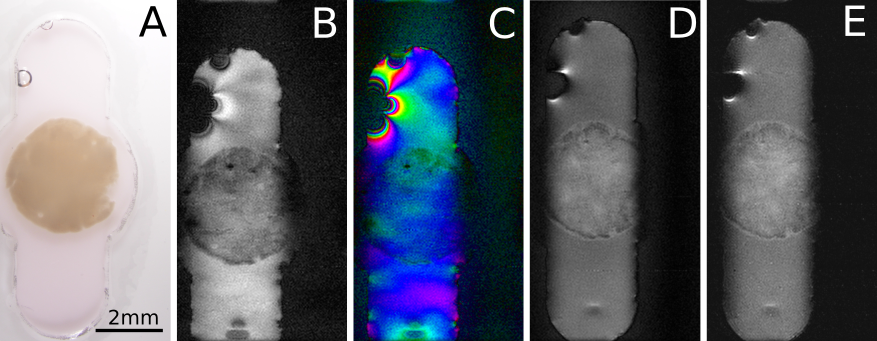
\includegraphics[width=.7\linewidth,keepaspectratio=true]{./figures/ms5n17-tisli-im-180511.png} 
\caption{MR images of a freshly cut live slice from a mouse. A: optical micrograph; B: Gradient echo image acquired in 1 minute; C: magnetic field map; D Spin echo image acquired in 30 minutes; E: RARE8 image acquired in 8 minutes.}
\label{fig:tisli} 
\end{figure}
%%%%%%%%%%%%%%%%%%%%%%%%%%%%%%%%%%%%%%%%%%%%%%%%%%%%%%%%%%%%%%%%%%
\section{Conclusions}
We have presented a novel modular NMR probe assembly for generic high sensitivity microfluidic NMR experiments. The probe is built from the readily accessible materials with no requirement of parts from commercial probes. The modularity of the probe enables to use different detectors tailored for specific experimental requirements on the same probe skeleton. The detector is made from easily available PCB materials. The use of PCB allows to modify the probe circuit and design without disturbing the probe geometry. The probe has excellent B$_1$ homogeneity and sensitivity. The resolution is reasonable for primary metabolic studies but needs to be improved for generic applications. The probe has already been used for various diverse experiments like reaction monitoring, protein structure determination, micro-imaging of mouse liver tissue slices, metabolic studies of mammalian cells, hyperpolarisation on the chip etc. Although in the current form the probe can be used for generic 2D experiments, in the future we intend to include extra channels for lock and pulses on other nuclei. Though, commercial gradient system has been successful to make micro images of mouse liver tissue slices, a dedicated gradient system can be included on the probe PCB for shimming and imaging.
%%%%%%%%%%%%%%%%%%%%%%%%%%%%%%%%%%%%%%%%%%%%%%%%%%%%%%%%%%%%%%%%%%
\section{Acknowledgement}
This research was funded through "Future and Emerging Technologies" (FETOPEN) call of the EU Horizon 2020 research framework. Authors would like to thank William Hale and Bishnubrata Patra for making microfluidic devices and Dr. Katrin Deinhardt from Department of Biological Science at UoS, for the mouse liver tissue..
%%%%%%%%%%%%%%%%%%%%%%%%%%%%%%%%%%%%%%%%%%%%%%%%%%%%%%%%%%%%%%%%%%
\clearpage
\bibliographystyle{unsrt}
\bibliography{science}
\end{document}